\documentclass{standalone}
\usepackage{tikz}
\usetikzlibrary{patterns}
\usetikzlibrary{positioning}
\usetikzlibrary{patterns, positioning}
\usetikzlibrary{shapes.misc}
\usepackage[outline]{contour}
\contourlength{1.5pt} 
\usetikzlibrary{calc}
        \usepackage{relsize}
        \tikzset{fontscale/.style = {font=\relsize{#1}}}

\begin{document}
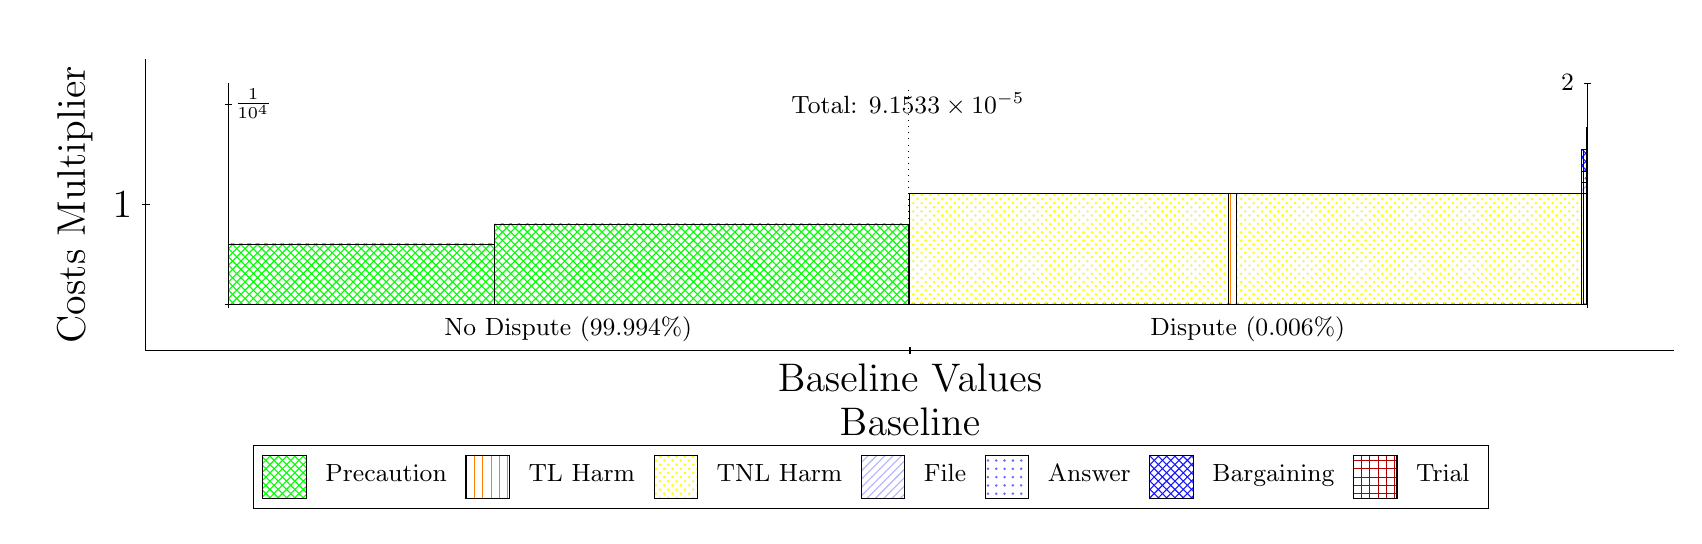
\begin{tikzpicture}
\clip(-0.5,-1.1) rectangle +(20.91,6.2);
\draw[black] (1,1) -- (1,4.7);
\node[rotate=90, fontscale=2, anchor=center] at (0.1, 2.85) {Costs Multiplier};
\draw[black] (0.95,2.85) -- (1.05,2.85);
\node[fontscale=2, anchor=east] at (0.95, 2.85) {1};

\draw[black] (1,1) -- (20.41,1);
\node[fontscale=2, anchor=center] at (10.705, 0.1) {Baseline};
\draw[black] (10.705,0.95) -- (10.705,1.05);
\node[fontscale=2, anchor=north] at (10.705, 0.95) {Baseline Values};


\draw[pattern=crosshatch, pattern color=green,draw=black,very thin] (2.05,1.592) rectangle (5.4319,2.354);
\draw[pattern=crosshatch, pattern color=green,draw=black,very thin] (5.4319,1.592) rectangle (10.68,2.608);
\draw[pattern=crosshatch, pattern color=green,draw=black,very thin] (10.68,1.592) rectangle (10.692,1.592);
\draw[pattern=north east lines, pattern color=blue!30,draw=black,very thin] (10.68,1.592) rectangle (10.692,1.7324);
\draw[pattern=dots,  pattern color=blue!60,draw=black,very thin] (10.68,1.7324) rectangle (10.692,1.8728);
\draw[pattern=crosshatch,      pattern color=blue!90,draw=black,very thin] (10.68,1.8728) rectangle (10.692,2.1536);
\draw[pattern=crosshatch, pattern color=green,draw=black,very thin] (10.692,1.592) rectangle (14.748,1.592);
\draw[pattern=crosshatch dots, pattern color=yellow,draw=black,very thin] (10.692,1.592) rectangle (14.748,2.996);
\draw[pattern=crosshatch, pattern color=green,draw=black,very thin] (14.748,1.592) rectangle (14.846,1.592);
\draw[pattern=vertical lines, pattern color=orange,draw=black,very thin] (14.748,1.592) rectangle (14.846,2.996);
\draw[pattern=crosshatch, pattern color=green,draw=black,very thin] (14.846,1.592) rectangle (19.227,1.5921);
\draw[pattern=crosshatch dots, pattern color=yellow,draw=black,very thin] (14.846,1.5921) rectangle (19.227,2.996);
\draw[pattern=crosshatch, pattern color=green,draw=black,very thin] (19.227,1.592) rectangle (19.258,1.592);
\draw[pattern=crosshatch dots, pattern color=yellow,draw=black,very thin] (19.227,1.592) rectangle (19.258,2.996);
\draw[pattern=north east lines, pattern color=blue!30,draw=black,very thin] (19.227,2.996) rectangle (19.258,3.1364);
\draw[pattern=dots,  pattern color=blue!60,draw=black,very thin] (19.227,3.1364) rectangle (19.258,3.2768);
\draw[pattern=crosshatch,      pattern color=blue!90,draw=black,very thin] (19.227,3.2768) rectangle (19.258,3.5576);
\draw[pattern=crosshatch, pattern color=green,draw=black,very thin] (19.258,1.592) rectangle (19.296,1.592);
\draw[pattern=vertical lines, pattern color=orange,draw=black,very thin] (19.258,1.592) rectangle (19.296,2.996);
\draw[pattern=north east lines, pattern color=blue!30,draw=black,very thin] (19.258,2.996) rectangle (19.296,3.1364);
\draw[pattern=dots,  pattern color=blue!60,draw=black,very thin] (19.258,3.1364) rectangle (19.296,3.2768);
\draw[pattern=crosshatch,      pattern color=blue!90,draw=black,very thin] (19.258,3.2768) rectangle (19.296,3.5576);
\draw[pattern=crosshatch, pattern color=green,draw=black,very thin] (19.296,1.592) rectangle (19.307,1.592);
\draw[pattern=crosshatch dots, pattern color=yellow,draw=black,very thin] (19.296,1.592) rectangle (19.307,2.996);
\draw[pattern=north east lines, pattern color=blue!30,draw=black,very thin] (19.296,2.996) rectangle (19.307,3.1364);
\draw[pattern=dots,  pattern color=blue!60,draw=black,very thin] (19.296,3.1364) rectangle (19.307,3.2768);
\draw[pattern=crosshatch,      pattern color=blue!90,draw=black,very thin] (19.296,3.2768) rectangle (19.307,3.5576);
\draw[pattern=grid,            pattern color=red!70!black,draw=black,very thin] (19.296,3.5576) rectangle (19.307,3.8384);
\draw[pattern=crosshatch, pattern color=green,draw=black,very thin] (19.307,1.592) rectangle (19.31,1.592);
\draw[pattern=vertical lines, pattern color=orange,draw=black,very thin] (19.307,1.592) rectangle (19.31,2.996);
\draw[pattern=north east lines, pattern color=blue!30,draw=black,very thin] (19.307,2.996) rectangle (19.31,3.1364);
\draw[pattern=dots,  pattern color=blue!60,draw=black,very thin] (19.307,3.1364) rectangle (19.31,3.2768);
\draw[pattern=crosshatch,      pattern color=blue!90,draw=black,very thin] (19.307,3.2768) rectangle (19.31,3.5576);
\draw[pattern=grid,            pattern color=red!70!black,draw=black,very thin] (19.307,3.5576) rectangle (19.31,3.8384);
\node[font=\small,text=black,anchor=north] at (10.68, 4.4) {Total: $9.1533\times 10^{-5}$};
\draw[black,very thin] (2.05,1.592) -- (2.05,4.4);
\draw[black,very thin] (2,1.592) -- (2.1,1.592);
\node[font=\small,text=black, anchor=west] at (2, 1.592) {};
\draw[black,very thin] (2,4.1321) -- (2.1,4.1321);
\node[font=\small,text=black, anchor=west] at (2, 4.1321) {$\frac{1}{10^{4}}$};

\draw[black,dotted,very thin] (10.68,1.6762) -- (10.68,4.3158);
\draw[black,very thin] (19.31,1.592) -- (19.31,4.4);
\draw[black,very thin] (19.26,4.3999) -- (19.36,4.3999);
\node[font=\small,text=black, anchor=east] at (19.26, 4.3999) {\contour{white}{2}};

\draw[black,very thin] (2.05,1.592) -- (19.31,1.592);
\draw[black,very thin] (2.05,1.542) -- (2.05,1.642);
\node[font=\small,text=black, anchor=north] at (2.05, 1.542) {};
\draw[black,very thin] (19.31,1.542) -- (19.31,1.642);
\node[font=\small,text=black, anchor=north] at (19.31, 1.542) {};

\node[font=\small,text=black,anchor=south] at (6.365, 0.992) {No\ Dispute\ (99.994\%)};
\node[font=\small,text=black,anchor=south] at (14.995, 0.992) {Dispute\ (0.006\%)};

\coordinate (LegendAnchor) at (10.205000000000002,0);
\begin{scope}[align=center]
\matrix[scale=0.6,draw=black,below=0.2cm of LegendAnchor,nodes={draw},column sep=0.12cm]{
\node[rectangle,draw,minimum width=0.55cm,minimum height=0.55cm,pattern=crosshatch, pattern color=green]{}; &
        \node[draw=none,font=\small]{Precaution}; &
\node[rectangle,draw,minimum width=0.55cm,minimum height=0.55cm,pattern=vertical lines, pattern color=orange]{}; &
        \node[draw=none,font=\small]{TL Harm}; &
\node[rectangle,draw,minimum width=0.55cm,minimum height=0.55cm,pattern=crosshatch dots, pattern color=yellow]{}; &
        \node[draw=none,font=\small]{TNL Harm}; &
\node[rectangle,draw,minimum width=0.55cm,minimum height=0.55cm,pattern=north east lines, pattern color=blue!30]{}; &
        \node[draw=none,font=\small]{File}; &
\node[rectangle,draw,minimum width=0.55cm,minimum height=0.55cm,pattern=dots, pattern color=blue!60]{}; &
        \node[draw=none,font=\small]{Answer}; &
\node[rectangle,draw,minimum width=0.55cm,minimum height=0.55cm,pattern=crosshatch, pattern color=blue!90]{}; &
        \node[draw=none,font=\small]{Bargaining}; &
\node[rectangle,draw,minimum width=0.55cm,minimum height=0.55cm,pattern=grid, pattern color=red!70!black]{}; &
        \node[draw=none,font=\small]{Trial}; \\
};\end{scope}

\end{tikzpicture}
\end{document}